\let\negmedspace\undefined
\let\negthickspace\undefined
\documentclass[journal]{IEEEtran}
\usepackage[a5paper, margin=10mm, onecolumn]{geometry}
%\usepackage{lmodern} % Ensure lmodern is loaded for pdflatex
\usepackage{tfrupee} % Include tfrupee package

\setlength{\headheight}{1cm} % Set the height of the header box
\setlength{\headsep}{0mm}     % Set the distance between the header box and the top of the text

\usepackage{gvv-book}
\usepackage{gvv}
\usepackage{cite}
\usepackage{amsmath,amssymb,amsfonts,amsthm}
\usepackage{algorithmic}
\usepackage{graphicx}
\usepackage{textcomp}
\usepackage{xcolor}
\usepackage{txfonts}
\usepackage{listings}
\usepackage{enumitem}
\usepackage{mathtools}
\usepackage{gensymb}
\usepackage{comment}
\usepackage[breaklinks=true]{hyperref}
\usepackage{tkz-euclide} 
\usepackage{listings}
% \usepackage{gvv}                                        
\def\inputGnumericTable{}                                 
\usepackage[latin1]{inputenc}                                
\usepackage{color}                                            
\usepackage{array}                                            
\usepackage{longtable}                                       
\usepackage{calc}                                             
\usepackage{multirow}                                         
\usepackage{hhline}                                           
\usepackage{ifthen}                                           
\usepackage{lscape}
\begin{document}

\bibliographystyle{IEEEtran}
\vspace{3cm}

\title{
1-Vector Arithmetic \\
\large EE1030:Matrix Theory
}
\author{Gajjarapu Satyanarayana\\AI24BTECH11009
}
% \maketitle
% \newpage
% \bigskip
{\let\newpage\relax\maketitle}

\renewcommand{\thefigure}{\theenumi}
\renewcommand{\thetable}{\theenumi}



\numberwithin{equation}{enumi}
\numberwithin{figure}{enumi}
\renewcommand{\thetable}{\theenumi}


\textbf{Question}:1.3.3\\
Points \textbf{A}(3,1), \textbf{B}(5,1), \textbf{C}($a,b$), \textbf{D}(4,3) are vertices of a parallelogram ABCD.Find the values of $a$ and $b$.\hfill(10,2019)
\\
\textbf{Solution:}
\renewcommand{\tablename}{Table 1.3.3.1}
\begin{table}[h!]
  \centering
  \begin{tabular}[12pt]{ |c| c|}
    \hline
    \textbf{Vertex} & \textbf{Coordinates}\\ 
    \hline
    \textbf{A} & \myvec{3 \\ 1} \\
    \hline 
    \textbf{B} & \myvec{5 \\ 1}\\
    \hline
    \textbf{C} & \myvec{a \\ b}\\
    \hline
    \textbf{D} & \myvec{4 \\ 3}\\
    \hline
    \end{tabular}

  \caption{Vertex and its coordinates}
\end{table}\\
 If ABCD is a parallelogram then,
 \begin{align}
     \textbf{B} - \textbf{A} = \textbf{C} - \textbf{D} \label{eq1.3.3.1} \\
     \textbf{B} - \textbf{A} = \myvec{5 \\ 1} - \myvec{3 \\ 1} \\
     \textbf{B} - \textbf{A} = \myvec{5 - 3 \\ 1 - 1}\\
     \textbf{B} - \textbf{A} = \myvec{2 \\ 0} \label{eq1.3.3.2} \\
	 \textbf{C} - \textbf{D} = \myvec{a \\ b} - \myvec{3 \\ 3} \\
     \textbf{C} - \textbf{D} = \myvec{a - 4 \\ 3 - b} \label{eq1.3.3.3} \\
     \end{align}
Since  \textbf{B} - \textbf{A} = \textbf{C} - \textbf{D} from equation \ref{eq1.3.3.1} , compare both the equations \ref{eq1.3.3.2} and \ref{eq1.3.3.3} \\
Therefore,
\begin{align}
    \myvec{2 \\ 0} = \myvec{a - 4 \\ b - 3} \\
\end{align}
Comparing similar terms,
\begin{align}
    2 = a - 4 \label{eq1.3.3.4} \\
    0 = b - 3 \label{eq1.3.3.5}
\end{align}
From equations \ref{eq1.3.3.4} and \ref{eq1.3.3.5} , \\
\begin{align}
    a = 6 \\
    b = 3
    \end{align}
    \begin{figure}[h!]
	    \centering
	    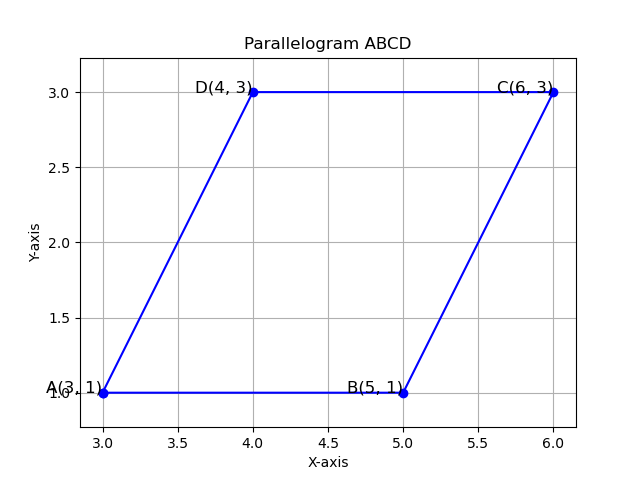
\includegraphics[width=0.7\linewidth]{figs/pgm.png}
	    \caption{Plot of the Parallelogram}
    \end{figure}
    \end{document}
